\chapter{Разработка алгоритмов управления БОЭП} \label{ch:ch4}

Объектом исследования является системы автоматического управления (САУ) оптико-электронным прибором (ОЭП) в пространстве по азимуту и углу места в режимах наведения и стабилизации.

Цель работы – является разработка компьютерной имитационных моделей изолированных каналов управления ОЭП, управляемого моментными двигателями по азимуту и углу места и исследование его динамических свойств.
В процессе работы проводились выбор моментных двигателей, синтез алгоритмов управления, разработка компьютерных имитационных моделей изолированных нелинейных каналов управления бортового ОЭП и исследование динамики управления им в режимах наведения и стабилизации.

В результате исследования динамики предложены алгоритмы управления и требования к структуре и элементам изолированных каналов управления, обеспечивающие требования ТЗ, которые будут уточнены при исследовании пространственной задачи управления.

Эффективность управления в режиме наведения достигается применением оптимального управления по быстродействию. 
Все расширяющийся круг военных и гражданских задач, для решения которых широко используются оптико-электронные методы и средства, вызвало интерес к решению научно- технических   проблем, возникающих при решении этих задач \cite[]{Tarasov}, \cite[]{Fedoseev}.

Одна из важных проблем – это влияние динамики и управления на достижение требуемых тактико- технических характеристик бортовых ОЭП и комплексов. Вопросы разработки, моделирования и исследования динамических систем, в том числе бортовых оптико-электронных комплексов, отражены в трудах международных Четаевских конференций по аналитической механике, устойчивости и управлению; в трудах международных симпозиумов по автоматическому управлению и всесоюзных совещаниях по теории инвариантности, в трудах КАИ, а также в журналах: «Оптический журнал», «Гироскопия и навигация», «Оптико-механическая промышленность», «Автоматика и телемеханика», «Авиационная техника», «Вестник КГТУ им. А. Н. Туполева» [4-26]. Разработке алгоритмов и исследованию динамики, и управлению посвящены работы [3 - 29].

На данном этапе разработки выполняемой НИР проведены предварительные расчеты по уяснению решаемых задач и анализу исходных данных, оговоренных техническим заданием (ТЗ), разработке и согласованию
расчетных оптико – механической схем и параметров ОЭП, приводов, датчиков угла САУ с учетом их технических требований и внешних воздействий от носителя.


\section{Технические требования и режимы управления ОЭП} \label{ch:ch4/sect1}

В соответствии с требованиями ТЗ были проанализированы, уточнены, доопределены следующие исходные данные, необходимые для расчета:
\begin{itemize}
	\item Состав системы автоматического управления,
	\item САУ по азимуту,
	\item САУ по углу места,
	\item Датчики углового положения по азимуту и углу места,
	\item Двигатели типа ДБМ (уточняются в процессе разработки) по азимуту и углу места,
	\item Усилительно-преобразовательные блоки каналов управления совместно с микропроцессорными блоками,
	\item Назначение и технические требования.
\end{itemize}
САУ предназначена для наведения оси визирования на заданные угловые координаты относительно строительных осей летательного аппарата (ЛА), параметры движения ЛА.

\newpage
%%%%%%%%%%%%%%%%%%%% Table No: 9 starts here %%%%%%%%%%%%%%%%%%%%

\begin{table}[!h]
	\caption{Технические параметры САУ}%
	\label{tab:SAU_PARAM}% label всегда желательно идти после caption
	\begin{longtable}{|m{5cm}|m{5.5cm}|m{5.5cm}|}
		\hline
		& по азимуту & по углу места \\ 
\hline
Пределы наведения		& $\pm$ 180 град           & (-60 .. +30) град              \\ 
\hline
Максимальная скорость наведения		&600 град/сек            &300 град/сек               \\ 
		\hline
Максимальная среднеквадратическая погрешность наведения и стабилизации		&<30 угловых минут           &<30 угловых минут               \\ 
		\hline
Время наведения на предельный угол		&<0.6 с            & <0.6 с              \\ 
		\hline
Синусоидальные вибрации		& \multicolumn{2}{m{11cm}|}{
	\begin{tabular}[l]{m{11cm}}
		Частота 5-10 Гц, амплитуда перемещения 5 мм\\
		Частота 20-22 Гц, ускорение $25 \textit{м/с}^2$\\
		Частота 35,4-50 Гц, амплитуда перемещения 0.5 мм\\
		Частота 50-500 Гц, ускорение $25 \textit{м/с}^2$
	\end{tabular}

}      \\ 
		\hline
Требования к САУ при внешних воздействиях		& \multicolumn{2}{m{11cm}|}{\begin{tabular}[l]{m{11cm}}
		максимальной скорости движения носителя – 56 м/с (200км/час)\\
		максимальный крен ЛА $\leq 15^0$\\
		угловая скорость носителя $\omega_y=12$ град/c\\
		минимальная высота полета носителя – 1500 м\\
		максимальная скорость движения ОН – 500 м/с	
\end{tabular}}      \\ 
		\hline
Гармонические возмущения, идущие от ЛА по азимуту и углу места		& \multicolumn{2}{m{11cm}|}{\begin{tabular}[l]{m{11cm}}
		Частота 0.16 Гц, амплитуда колебаний 12 град.\\
		Частота 1 Гц, амплитуда колебаний 1- 2 град.
\end{tabular}}      \\ 
		\hline
Требования к САУ при воздействиях ускорений в условиях движения носителя		& \multicolumn{2}{m{11cm}|}{$4.8 \textit{м/с}^2$}      \\ 
		\hline
	\end{longtable}
\end{table}

%%%%%%%%%%%%%%%%%%%% Table No: 9 ends here %%%%%%%%%%%%%%%%%%%%

Геометрия масс тел вращения объекта управления (ОУ) по двум осям управления опредставлена в таблице \ref{tab:MASS/3.1} и рисунокe \ref{fig:41}.

%%%%%%%%%%%%%%%%%%%% Figure/Image No: 30 starts here %%%%%%%%%%%%%%%%%%%%

\begin{figure}[!ht]
	\centering
	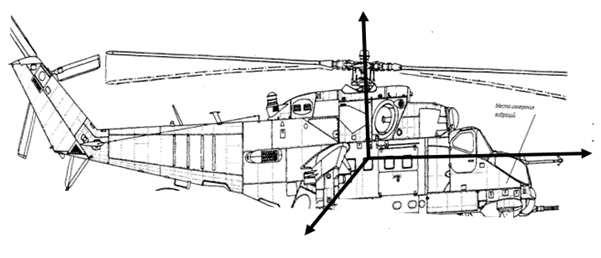
\includegraphics[width=0.8\linewidth]{img-25} 
	\caption{Обозначение строительных осей ЛА}
	\label{fig:41}
\end{figure}

%%%%%%%%%%%%%%%%%%%% Figure/Image No: 30 Ends here %%%%%%%%%%%%%%%%%%%%

В отчете приведены синтез алгоритмов управления, разработка компьютерных моделей и исследование динамики изолированных каналов управления САУ с учетом частоты ШИМ и насыщения усилителей мощности, дискретизации датчиков угла.


\section{Обоснование выбора приводов} \label{ch:ch4/sect2}

Требуемая мощность и развиваемый момент двигателя определяются по формулам \cite[]{Bessekerski}:\par


\begin{equation}
	\label{eq:p4:1}
	\begin{multlined}
P \geq 2 \left( M_{\textit{нагр}}+I_{\textit{нагр}} \ddot \alpha^{max}   \right) \dot \alpha^{max},\\
M_{\textit{дв}} \geq 2 \left[ M_{\textit{нагр}}+I_{\textit{нагр}} \ddot \alpha^{max}  \right], \\
M_{\textit{нагр}}=M_{\textit{тр}}+M_{\textit{дб}}.
\end{multlined}
\end{equation}

Здесь 
$P$ - мощность двигателя, 
$М_{\textit{дв}}$ – момент на валу двигателя, 
$M_{\textit{нагр}}$ - статический момент нагрузки, 
$I_{\textit{нагр}}$ - момент  инерции нагрузки, 
$М_{\textit{тр}}$ - момент трения на валу двигателя,
$М_{\textit{дб}}$ - момент дисбаланса нагрузки,  
$\ddot \alpha^{max}, \dot \alpha^{max}$ - максимальные угловые скорость и ускорение.\par

Оценим указанные параметры двигателей. 
В соответствии с требованиями ТЗ следует, что наиболее энергоемким является режим наведения. Ставится задача перевода оптической оси ОЭП относительно строительных осей ЛА за время \textit{0.6 с}. из одного положения в другое в пределах углов: по азимуту – $2 \alpha_0 = 360$ град., по углу места – $2 \beta_0 = 90$ град.  \par

Для решения этой задачи рассмотрим оптимальное управление по быстродействию (по минимуму времени перевода оптической оси ОЭП из одной точки пространства в другую) \cite[]{Babaev},\cite[]{Boltanski}. Суть такого управления состоит в том, что для перевода оптической оси на требуемый угол за минимальное время необходимо в первой половине этого времени разгоняться с постоянным положительным ускорением, а в другой половине – тормозить с постоянным отрицательным ускорением. Таким образом изменение угла поворота ОЭП будет проходить по нелинейной траектории (двум параболам).\par

Требуемое угловые ускорение и скорость ротора моментного двигателя с нагрузкой по азимуту, необходимое для достижения необходимого половинного угла $2 \beta_0 = 45$ град. за время $\tau=0.3$ с:\par

\begin{equation}
\label{eq:p4:1+}
\begin{multlined}
  \alpha _{0} = \frac{ \ddot \alpha _{0} \tau^{2}}{2} \rightarrow 
\ddot \alpha _{0} = \frac{2 \alpha _{0}}{ \tau^{2}} = \frac{2 \pi /2}{  0.3^{2}} = 34.906 \textit{рад/с}^{2},\\
\dot \alpha ^{max}= \ddot \alpha _{0} \tau = 34.906\cdot 0.3=10.47 \textit{рад/с}. 
\end{multlined}
\end{equation}

Требуемое угловые ускорение и скорость ротора моментного двигателя с нагрузкой по углу места, необходимое для достижения необходимого половинного угла $\beta_0=45$ град. за время $\tau=0.3$ с:

\begin{equation}
\label{eq:p4:1+1}
\begin{multlined}
\beta _{0} = \frac{ \ddot \beta _{0} \tau^{2}}{2} \rightarrow 
\ddot \beta _{0} = \frac{2 \beta _{0}}{ \tau^{2}} = \frac{2 \pi /4}{  0.3^{2}} = 17.453 \textit{рад/с}^{2},\\
\dot \beta ^{max}= \ddot \beta _{0} \tau = 17.453\cdot 0.3=5.235 \textit{рад/с}. 
\end{multlined}
\end{equation}
Моменты трения оценим по формуле:

\begin{equation}%\tag{44}
\label{eq:p4:4}
\begin{multlined}
	M_{\textit{тр}}= \left( 2  \div 5 \right) m 10^{-3} \left[ \textit{Нм} \right] 
\end{multlined}
\end{equation}
где \textit{m} – масса подвижной части прибора. С учетом данных из таблицы \ref{tab:MASS/3.1} (m1=15.7 кг, m2=1.131 кг) находим по формуле 41):\par

\begin{equation}%\tag{44}
\label{eq:p4:4+}
\begin{multlined}
M_{\textit{ТР1}} = 5 \cdot 10^{-3}\cdot 15.7 = 0.0785 \textit{Нм},\\
M_{\textit{ТР2}} = 5 \cdot 10^{-3}\cdot 1.131 = 0.005755 \textit{Нм}
\end{multlined}
\end{equation}

Моменты дисбаланса нагрузки определим по формулам:
\begin{equation}%\tag{44}
\label{eq:p4:4+1}
\begin{multlined}
М_{\textit{дб1}} = 
m_{1} \left( a+g \right) \sqrt[]{x_{c1}^{2}+y_{c1}^{2}} =
15.7 \left( 4.8 + 9.8 \right) \cdot 9 \cdot 10^{-3}=2.06 \textit{Нм},\\
М_{\textit{дб2}}=
m_{2} \left( a+g \right) у_{с2}=
1.131 \cdot 14.8 \cdot 10^{-3} = 0.245 \textit{Нм},
\end{multlined}
\end{equation}

здесь \textit{а }– ускорение, создаваемое носителем, \textit{g} – ускорение земного притяжения, \textit{х\textsubscript{с1},у\textsubscript{с1},у\textsubscript{с2}} – величины дисбаланса ОЭП (таблица \ref{tab:MASS/3.1})\par

Максимальные статические моменты нагрузки на валу двигателей по азимуту и углу места соответственно равны:\par

\begin{equation}%\tag{44}
\label{eq:p4:4+2}
\begin{multlined}
M_{\textit{нагр1}}=M_{\textit{ТР1}}+M_{\textit{дб1}}=0.078+2.064=2.1425 \textit{Нм}, \\
M_{\textit{нагр2}}=0.005755+0.245=0.250755 \textit{Нм}.
\end{multlined}
\end{equation}

В результате получили следующие исходные данные для расчета требуемых моментов и мощностей на валу двигателей:\par


	\begin{tabular}{ll}
\( \ddot \alpha _{0}=34,9\textit{рад/с}^{2} \)				& \( \ddot \beta _{0}=17.45 \textit{рад/с}^{2} \)  \\
\( I_{y}=0.327\textit{кгм}^{2} \)						&  \( I_{z}=0.0084 \textit{кгм}^{2} \) \\
\( m_{1}=15.7\textit{кг} \)								& \( m_{2}=1.131 \textit{кг} \) \\
\( \dot \alpha ^{max}=10.47\textit{рад/с} \)				& \( \dot \beta ^{max}=5.235\textit{рад/с} \) \\
\( M_{\textit{\textit{нагр1}}}=2.1425\textit{Нм} \)		& \( M_{\textit{\textit{нагр2}}}=0.250755\textit{Нм} \)
	\end{tabular}


В силу (\labelcref{eq:p4:1}) получим требования к двигателям по азимуту и углу места:\par

- к пусковому моменту на валу ротора

\begin{equation}%\tag{44}
\label{eq:p4:4+3}
\begin{multlined}
M_{\textit{дв1}} \geq 2 \left[ 2.1425 + \left( 0.327 \cdot 34.9 \right)  \right] =27.1096\textit{Нм} \rightarrow 30\textit{Нм}, \\
M_{\textit{дв2}} \geq 2 \left[ 0.25 + 0.0084 \cdot 17.45 \right] =0.79316\textit{Нм} \rightarrow 1\textit{Нм};
\end{multlined}
\end{equation}

- к потребляемой мощности

\begin{equation}%\tag{44}
\label{eq:p4:4+4}
\begin{multlined}
P_{1}=27.11 \cdot 10.47=283.84\textit{Вт} \rightarrow 300\textit{Вт}, \\
P_{2}=0.8 \cdot 5.235=4.2\textit{Вт} \rightarrow  \left( 5 \div 10 \right) \textit{Вт}.
\end{multlined}
\end{equation}
С учетом полученных требований можно использовать наиболее приемлемые моментные двигатели (МД) типа ДБМ (согласованные с Заказчиком) для управления ОЭП:

\begin{itemize}
	\item \textit{по азимуту}: 5\ ДБМ 120-5-2-3 (с запасом по пусковому моменту, новая разработка с 2007г.)  и 5 ДБМ 120-2-1-3 (без запаса по пусковому моменту, новая разработка с 2007г.), ДБМ 150-4-0,6-3 (без запаса по пусковому моменту, серийный с 2005г.), ДБМ 150-4-1,5-3 (с запасом по пусковому моменту, серийный с 2005г.)
	\item \textit{по углу места} – 3 ДБМ 70-1,1-1,3-3 (с запасом по пусковому моменту, серийный с 2005г.)
\end{itemize}

Характеристики указанных моментных двигателей приведены в таблице \ref{tab:DBM}. \par

\begin{landscape}


%%%%%%%%%%%%%%%%%%%% Table No: 10 starts here %%%%%%%%%%%%%%%%%%%%


\begin{table}[!h]
	\caption{Характеристики приводов ДБМ}%
	\label{tab:DBM}% label всегда желательно идти после caption
	\begin{longtable}{|m{10cm}|m{2.2cm}|m{2.2cm}|m{2.2cm}|m{2.2cm}|m{2.2cm}|m{2.2cm}|}
		\hline
		%row no:1
		Название & 
		5ДБМ120- 5-2-3 & 
		{3ДБМ120- \par 1-0.8-3} & 
		{5ДБМ120- \par 2-1-3} & 
		{3ДБМ150- \par 4-0.6-3} & 
		{ДБМ150- \par 4-1.5-3} & 
		{3ДБМ70- \par 1.1-1.3-3} \\
		\hline
		%row no:2
		Наружный диаметр статора, мм & 
		120 & 
		{120} & 
		{120} & 
		{150} & 
		{150} & 
		{70} \\
		\hline
		%row no:3
		Внутренний диаметр статора & 
		47 & 
		{} & 
		{} & 
		{72} & 
		{72} & 
		{28} \\
		\hline
		%row no:4
		Число пар полюсов & 
		8 & 
		{8} & 
		{8} & 
		{8} & 
		{8} & 
		{8} \\
		\hline
		%row no:5
		Число фаз & 
		3 & 
		{3} & 
		{3} & 
		{3} & 
		{3} & 
		{3} \\
		\hline
		%row no:6
		Номинальное напряжение питания, В & 
		27 & 
		{18} & 
		{18} & 
		{27} & 
		{27} & 
		{27} \\
		\hline
		%row no:7
		Частота вращения холостого хода, об/мин & 
		2200-2500 & 
		{740-900} & 
		{1080} & 
		{560-700} & 
		{1720-1910} & 
		{1120-1420} \\
		\hline
		%row no:8
		Пусковой момент, Н$\ast$ м, не менее & 
		54 & 
		{6.5} & 
		{29.4} & 
		{26} & 
		{37.4} & 
		{5.5} \\
		\hline
		%row no:9
		Сопротивление фазы постоянному току, Ом & 
		0.029- 0.035 & 
		{0.63- 0.77} & 
		{0.123} & 
		{0.22- 0.27} & 
		{0.1- 0.13} & 
		{0.45- 0.52} \\
		\hline
		%row no:10
		Электромагнитная постоянная времени фазы, мс, не более & 
		 & 
		{} & 
		{} & 
		{1.2} & 
		{1.8} & 
		{0.4} \\
		\hline
		%row no:11
		Приведенные к фазе коэффициенты момента Cm, Н$\ast$ м/А ; ЭДС Ce, В$\ast$ с/рад & 
		0.0075-0.0085 & 
		{0.17-0.21} & 
		{11-0.14} & 
		{0.23-0.28} & 
		{0.09-0.1} & 
		{0.1-0.14} \\
		\hline
		%row no:12
		Момент инерции ротора, кг$\ast$ м\textsuperscript{2} & 
		0.75 10\textsuperscript{-5} & 
		{1 10\textsuperscript{-5}} & 
		{0.26 10\textsuperscript{-5}} & 
		{3 10\textsuperscript{-3}} & 
		{3 10\textsuperscript{-3}} & 
		{2.5 10\textsuperscript{-4 }} \\
		\hline
		%row no:13
		Момент сопротивления, Н$\ast$ м, не более & 
		0.6 & 
		{0.1} & 
		{0.16} & 
		{0.4} & 
		{0.4} & 
		{0.11} \\
		\hline
		%row no:14
		Предельный ток, А & 
		 & 
		{} & 
		{} & 
		{66} & 
		{165} & 
		{40} \\
		\hline
		%row no:15
		Электромеханическая постоянная времени, мс & 
		 & 
		{} & 
		{} & 
		{10} & 
		{14.3} & 
		{7} \\
		\hline
		%row no:16
		Масса, кг & 
		 & 
		{} & 
		{} & 
		{3} & 
		{3} & 
		{1.2} \\
		\hline
		%row no:17
		Материал магнитов & 
		Nd-FE-B & 
		{EN38S} & 
		{EN38S} & 
		{Nd-Fe-B} & 
		{Nd-Fe-B} & 
		{Nd-Fe-B} \\
		\hline
		
\end{longtable}
\end{table}
%%%%%%%%%%%%%%%%%%%% Table No: 10 ends here %%%%%%%%%%%%%%%%%%%%
\end{landscape}

\begin{figure}[ht]
	\centering
	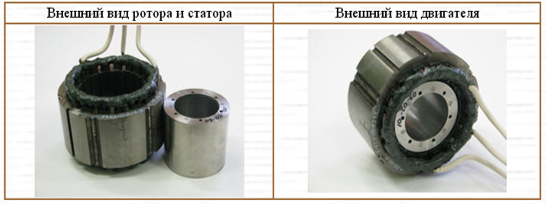
\includegraphics[width=0.8\linewidth]{image37} 
	\caption{Внешний вид 5ДБМ120- 5-2-3}
	\label{fig:5DBM120}
\end{figure}

\begin{figure}[ht]
	\centering
	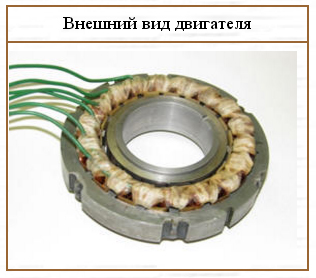
\includegraphics[]{image38} 
	\caption{Внешний вид 3ДБМ120-1-0.8-3, 5ДБМ120-2-1-3}
	\label{fig:3DBM120}
\end{figure}

\begin{figure}[ht]
	\centering
	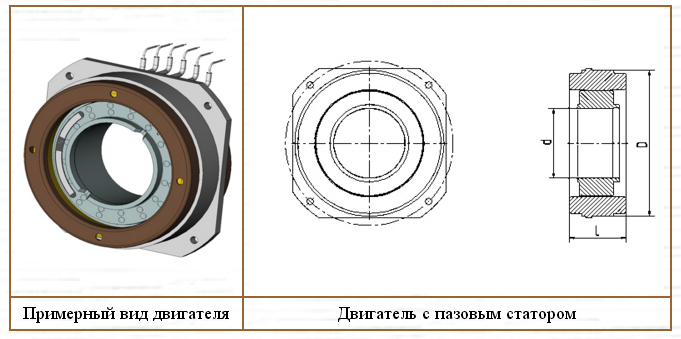
\includegraphics[width=0.8\linewidth]{image39} 
	\caption{Внешний вид 3ДБМ150-4-0.6-3, ДБМ150-4-1.5-3, 3ДБМ70-1.1-1.3-3}
	\label{fig:3DBM70}
\end{figure}

Для дальнейших исследований выбраны наиболее предпочтительные МД, удовлетворяющие требованиям ТЗ:\par

\begin{itemize}
	\item \textit{по азимуту} –  5ДБМ 120-5-2-3,
	\item \textit{по углу места} – 3 ДБМ 70-1,1-1,3-3.
\end{itemize}




\section{Уравнения движения изолированных каналов управления} \label{ch:ch4/sect3}

Используя линеаризованные уравнения (\ref{eq:p3:59}) полученные в разделе \ref{ch:ch3/sect10} составим зависимости положений приводов от управляющего сигнала, возмущающего воздействия и движений ЛА. В виду незначительного влияния перекрестных связей запишем уравнения (\ref{eq:p3:59}) в следующем виде:

\begin{equation}
\label{eq:p4:s3.1}
\begin{multlined}
\left( a_{11}p^{2}+b_{11}p \right)  \alpha + 
a_{11} p^2  \psi 
=
k_{1}  u_{1}- 
 M_{\textit{тр.1}},\\
\left( a_{22}p^{2}+b_{22}p \right)  \beta + c_{22}+
d_{23} p^2  \vartheta
=\\
k_{2}  u_{2} - M_{\textit{тр.2}},
\end{multlined}
\end{equation}

Перепишем уравнения относительно обобщенных координат:

\begin{equation}
\label{eq:p4:s3.2}
\begin{multlined}
\alpha= 
\frac{k_{1}}{a_{11}p^{2}+b_{11}p} u_{1} - 
\frac{1}{a_{11}p^{2}+b_{11}p} M_{\textit{тр.1}} - 
\frac{a_{11} p^2}{a_{11}p^{2}+b_{11}p}  \psi  ,\\
\beta=
\frac{k_{2}}{a_{22}p^{2}+b_{22}p} u_{2} - 
\frac{1}{a_{22}p^{2}+b_{22}p} M_{\textit{тр.2}} - \\
\frac{d_{23} p^2}{a_{22}p^{2}+b_{22}p} \vartheta -
\frac{1}{a_{22}p^{2}+b_{22}p} c_{22},
\end{multlined}
\end{equation}

Из выражения (\ref{eq:p4:s3.2}) следует, что уголы поворота ОЭП зависит не только от управления, но и от моментов трения, дисбаланса ($c_{22}=M_{\textit{дб}}$) и движений носителя. Для дальнейшего использования выражение (\ref{eq:p4:s3.2}) запишем в виде:

\begin{equation}
\label{eq:p4:s3.3}
\begin{multlined}
\alpha= 
W_{n1}(p) u_{1} - 
W_{f1}(p) M_{\textit{тр.1}} - 
W_{\psi 1}(p)  \psi  ,\\
\beta=
W_{n2}(p) u_{2} - 
W_{f2}(p) (M_{\textit{дб}} + M_{\textit{тр.2}}) - 
W_{\vartheta}(p) \vartheta,
\end{multlined}
\end{equation}
где
ПФ азимута по управлению:
\begin{equation}
\label{eq:p4:s3.4}
\begin{multlined}
W_{n1}(p) = \frac{k_{1}}{a_{11}p^{2}+b_{11}p} = \frac{1}{C_{e1}} \frac{1}{(a_1 p^2 + b_1 p +1)p};
\end{multlined}
\end{equation}
ПФ азимута по возмущению:
\begin{equation}
\label{eq:p4:s3.5}
\begin{multlined}
W_{f1}(p) = \frac{1}{a_{11}p^{2}+b_{11}p} = \frac{R_1}{C_{m1}C_{e1}} \frac{(T_1 p +1)}{(a_1 p^2 + b_1 p +1)p};
\end{multlined}
\end{equation}
ПФ азимута от движения носителя:
\begin{equation}
\label{eq:p4:s3.6}
\begin{multlined}
W_{\psi}(p) = \frac{a_{11} p^2}{a_{11}p^{2}+b_{11}p} = b_1 \frac{(T_1 p +1)p}{(a_1 p^2 + b_1 p +1)};
\end{multlined}
\end{equation}
где 
$a_1 = \frac{L_1 (B_1 + B(\beta_0))}{C_{m1}C_{e1}} $,
$b_1 = \frac{R_1 (B_1 + B(\beta_0))}{C_{m1}C_{e1}} $,
$T_1 = R_1/L_1$

ПФ угла места по управлению:
\begin{equation}
\label{eq:p4:s3.7}
\begin{multlined}
W_{n2}(p) = \frac{k_{2}}{a_{22}p^{2}+b_{22}p} = \frac{1}{C_{e1}} \frac{1}{(a_2 p^2 + b_2 p +1)p};
\end{multlined}
\end{equation}
ПФ угла места по возмущению:
\begin{equation}
\label{eq:p4:s3.8}
\begin{multlined}
W_{f2}(p) = \frac{1}{a_{22}p^{2}+b_{22}p} = \frac{R_2}{C_{m2}C_{e2}} \frac{T_2 p + 1}{(a_2 p^2 + b_2 p +1)p};
\end{multlined}
\end{equation}
ПФ угла места от движения носителя:
\begin{equation}
\label{eq:p4:s3.9}
\begin{multlined}
W_{\vartheta}(p) = \frac{d_{23} p^2}{a_{22}p^{2}+b_{22}p} = 
\frac{R_2 d_{23}}{C_{m2}C_{e2}} \frac{(T_2 p + 1)p}{(a_2 p^2 + b_2 p +1)};
\end{multlined}
\end{equation}
где 
$a_2 = \frac{L_2 C_2}{C_{m2}C_{e2}} $,
$b_2 = \frac{R_1 C_2}{C_{m2}C_{e2}} $,
$T_2 = R_2/L_2$

\begin{comment}
\subsection{Уравнения движения привода по азимуту} \label{subsec:ch4/sect3/sub1}

Линеаризованные уравнения движения азимутального привода совместно с объектом управления запишутся [29] [30] [31] [32] [33] [34]:

\subsection{Уравнения движения привода по углу места} \label{subsec:ch4/sect3/sub2}
\end{comment}



\section{Синтез алгоритмов программного устройства} \label{ch:ch4/sect2+}

\subsection{Режим наведения} \label{subsec:ch4/sect2/sub1}

Режим наведения должен осуществляться в пределах заданых углов относительно ЛА ($\varDelta\alpha$) за время ($\varDelta t$). Для решения этой задачи управления рассмотрим оптимальное управление по быстродействию [3, 27].

Задача устройства состоит в том чтобы выдать оптимальную траекторию движения основываясь на следующих условиях:
\begin{enumerate}
	\item средняя скорость разворота должна удовлетворять требованиям ТУ: 
	$\frac{\varDelta\alpha}{\varDelta t}$
	\item скорость движения в начальный и конечным момент должна быть равна 0
	\item программный угол не должен выходить за заданые пределы
\end{enumerate}

Построим программное устройство (ПУ), предназначенное для выдачи требуемой программной траектории движения оптической оси на основе решения уравнений:
\begin{equation}
\label{eq:p4:2+.1}
\begin{alignedat}{2}
\varDelta\alpha = \dfrac{\ddot{\alpha}{\varDelta t}^2}{4}
\end{alignedat}
\end{equation}

Схема моделирования ПУ приведена на рисунке \ref{fig:model_control}. Фрагмент решения уравнений (\ref{eq:p4:2+.1}) приведен далее (рисунок \ref{fig:model_control_graph}).

\begin{figure}[ht]
	\centering
	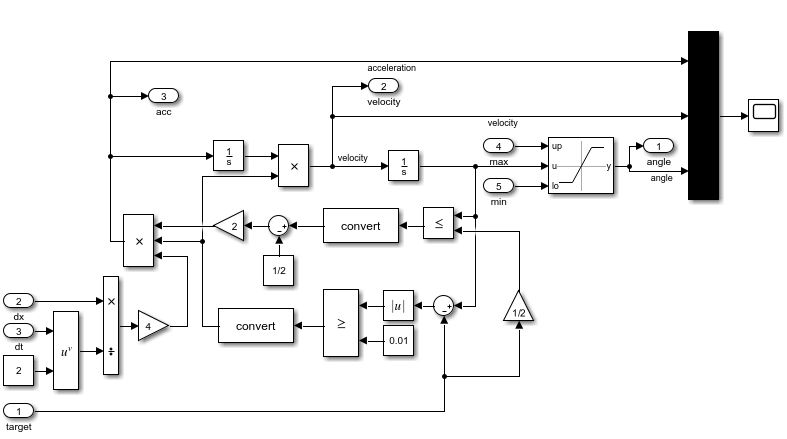
\includegraphics[width=1.0\linewidth]{model_control} 
	\caption{Схема моделирования программного устройства}
	\label{fig:model_control}
\end{figure}

Для задания необходимой программной траектории достаточно задать угол (обозначен как "target" на рисуноке \ref{fig:model_control}), на который  необходимо перевести оптическую ось ОЭП, задать скорость разворота (обозначен как "dx" и "dt" на рисуноке \ref{fig:model_control}) и задать предельные углы разворота (обозначен как "max" и "min" на рисуноке \ref{fig:model_control}). 

\begin{figure}
	\centering
	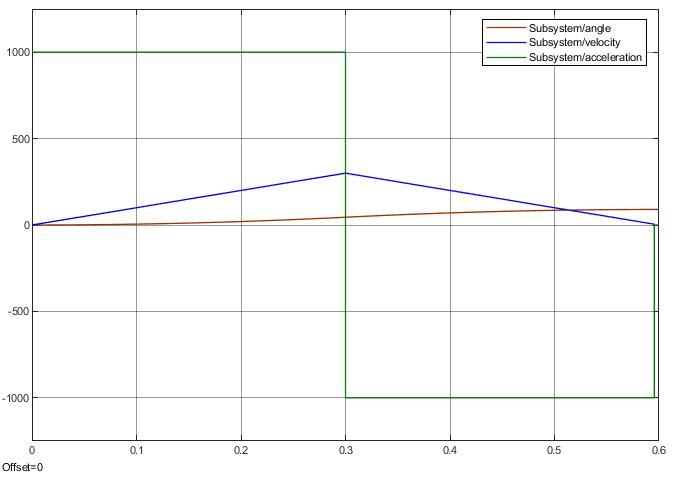
\includegraphics[width=0.7\linewidth]{model_control_graph}
	\caption{График ускорения, скорости и координаты программного движения}
	\label{fig:model_control_graph}
\end{figure}



\section{Синтез алгоритмов управления ОЭП} \label{ch:ch4/sect4-}

В соответствии с ТЗ управление ОЭП проводится в двух режимах:
наведения ОЭП на объект наблюдения (ОН) и стабилизации оптической оси относительно направления на ОН. 

Синтез алгоритмов управления проводился частотным методом [27] для каждого из режимов. На основе полученных законов управления разработаны компьютерные модели (КМ) линейной и нелинейной САУ в среде Simulink MatLAB и проведены исследования динамики САУ с помощью КМ в режимах наведения и стабилизации при действии возмущений, оговоренных в ТЗ.

Структурная схема САУ изолированного канала показана на рисунке \ref{fig:structured_SAU}.

\begin{figure}[ht]
	\centering
	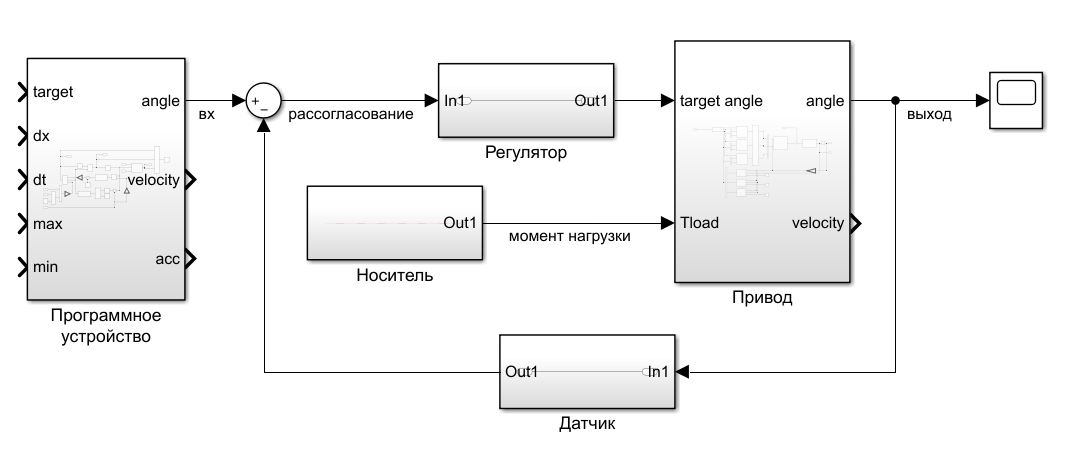
\includegraphics[width=0.8\linewidth]{structured_SAU}
	\caption{Структурная схема САУ}
	\label{fig:structured_SAU}
\end{figure}

Программное устройство определяет режим работы и задает целевое значение положения ротора канала, регулятор обеспечивает оптимальную работу привода, привод - объект управления , 
датчик угла измеряет положение ротора, "носитель" определяет внешние возмущающие факторы влияющие на систему.



\section{Синтез алгоритмов управления ОЭП, моделирование и исследование динамики САУ по азимуту в режиме наведения} \label{ch:ch4/sect4}


\subsection{Синтез и исследование линейной системы управления} \label{subsec:ch4/sect4/sub1}


\subsection{Синтез, моделирование и исследование динамики нелинейной САУ} \label{subsec:ch4/sect4/sub2}


\subsection{Синтез цифровых САУ } \label{subsec:ch4/sect4/sub3}


\subsection{Моделирование и исследование динамики ЦСАУ} \label{subsec:ch4/sect4/sub4}


\section{Синтез алгоритмов управления ОЭП, моделирование и исследование динамики САУ  по углу места  в режиме наведения} \label{ch:ch4/sect5}


\subsection{Синтез и исследование линейной САУ} \label{subsec:ch4/sect5/sub1}


\subsection{Синтез цифровых САУ } \label{subsec:ch4/sect5/sub2}


\subsection{Моделирование и исследование динамики ЦСАУ} \label{subsec:ch4/sect5/sub3}



\section{Моделирование и исследование динамики изолированных каналов управления ОЭП в режиме стабилизации} \label{ch:ch4/sect6}


\subsection{Моделирование и исследование динамики нелинейной САУ по курсу} \label{subsec:ch4/sect6/sub1}


\subsection{Моделирование и исследование динамики нелинейной САУ по углу места} \label{subsec:ch4/sect6/sub2}


\section{Анализ результатов исследований и определение требований к элементам САУ} \label{ch:ch4/sect7}


\section{Выводы по главе} \label{ch:ch4/sect8}



Некоторый текст.

\clearpage